%%
\documentclass[%
]{ittmm}


\usepackage{polyglossia}
\setdefaultlanguage[spelling=modern]{russian}
\setotherlanguages{english}

%%% One can fix some overfulls
\sloppy

%% Minted listings support
%% Need pygment <http://pygments.org/> <http://pypi.python.org/pypi/Pygments>
%\usepackage[newfloat]{minted}
\usepackage{minted}
%% auto break lines
\setminted{breaklines=true}

%\usepackage{caption}

%\newenvironment{code}{\captionsetup{type=listing}}{}
%\SetupFloatingEnvironment{listing}{name=Листинг}

\addbibresource{main.bib}

%% end of the preamble, start of the body of the document source.
\begin{document}

\selectlanguage{russian}

%%
%% Rights management information.
%% CC-BY is default license.
\copyrightyear{2025}
\copyrightclause{Copyright for this paper by its authors.
  Use permitted under Creative Commons License Attribution 4.0
  International (CC BY 4.0).}

%%
%% This command is for the conference information
\conference{Information and Telecommunication Technologies and Mathematical Modeling of High-Tech Systems 2025 (ITTMM 2025), Moscow, April 07--11, 2025}

%%
%% The "title" command
\title{Симулятор беспроводной меш-сети для мобильных роботов}
\title[mode=trans]{Wireless mesh network simulator for mobile robots}

% \tnotemark[1]
% \tnotetext[1]{You can use this document as the template for preparing your publication. We recommend using the latest version of the ittmm style.}

%%
%% The "author" command and its associated commands are used to define
%% the authors and their affiliations.
\author[1]{Даниил М. Генералов}[%
trans={Daniil M. Generalov},
orcid=0000-0002-2337-1176,
email=1032212280@pfur.ru,
%url=https://yamadharma.github.io/,
]
\cormark[1]

\address[1]{Российский университет дружбы народов, ул. Миклухо-Маклая, д. 6, Москва, 117198, Российская Федерация}

\author[1]{Андрей Н. Виноградов}[%
trans={Andrei N. Vinogradov},
email=vinogradov-an@rudn.ru,
orcid=0000-0002-3349-8859,
]

%%% Footnotes
\cortext[1]{Автор, отвечающий за публикацию.}

%%
%% The abstract is a short summary of the work to be presented in the
%% article.
\begin{abstract}
В этой работе мы представляем программу-симулятор
для разработки и тестирования алгоритмов маршрутизации
в беспроводных меш-сетях на мобильных роботах.
С помощью этого симулятора можно
изучать поведение этих мобильных роботов
при различных условиях радио-связи,
которые трудно симулировать на физическом оборудовании.
Код, написанный для симулятора,
можно использовать на физических микроконтроллерах без изменений.
Интеграция симуляции радио-связи
и движения роботов по прямоугольной сетке
является новым подходом,
который сложно воспроизвести в существующих инструментах симуляции сетей.
\end{abstract}

%%
%% Keywords. The author(s) should pick words that accurately describe
%% the work being presented. Separate the keywords with commas.
\begin{keywords}
  меш-сеть \sep
  MANET \sep
  маршрутизация \sep
  симулятор
\end{keywords}

%% This command processes the author and affiliation and title
%% information and builds the first part of the formatted document.
\maketitle

\section{Введение}
\label{sec:intro}

\subsection{Меш-сети}
Беспроводные меш-сети (MANET, \emph{Mobile Ad-hoc Network})
отличаются от традиционных радио-сетей тем,
что они не имеют центрального роутера (такого как Wi-Fi AP или сотовая базовая станция);
вместо этого каждый клиент сети является также роутером для своих соседей.

На таком принципе работают рации:
каждая рация может передать сигнал тем приемникам, которые находятся в ее радиусе действия.
Сообщения могут идти дальше, чем радиус действия одного сигнала,
посредством ретрансляции:
если Алиса хочет передать сообщение Чарли,
но Алиса находится слишком далеко от него,
то Алиса может передать свое сообщение Бобу,
и Боб сможет передать сообщение дальше --
либо напрямую к Чарли, если он находится в его радиусе,
либо кому-то еще, кто находится ближе к Чарли.

Такой способ подключения напоминает широкое устройство интернета:
там тоже нет центральных роутеров,
и вместо этого каждая автономная система (AS, \emph{Autonomous System})
имеет пир-соединения (\emph{peering}) с другими AS.
Для этого администраторы двух сетей
соединяют свои роутеры друг с другом
и настраивают свою сеть так, чтобы обе стороны
могли доставлять свои пакеты через другую AS.

Таким образом сети различных организаций составляют глобальную сеть.
Автономные системы обмениваются информацией о том, какие другие системы доступны им,
с помощью протокола BGP (Border Gateway Protocol),
и на основании этой информации их роутеры решают, куда отправлять приходящий им трафик.

Устройство в беспроводной меш-сети примерно аналогично автономной системе интернета.
Однако есть одно важное отличие:
настройка пир-соединений между AS выполняется вручную
по обоюдному согласию администраторов каждой AS,
требует создания физического подключения
и настройки роутеров внутри AS.
Напротив, в беспроводной меш-сети,
устройства могут двигаться относительно друг друга и менять свою сетевую конфигурацию динамически,
так что настройка соединений между устройствами и обмен информацией
должен происходить без участия человека.

Дополнительная сложность заключается в том, что
беспроводные меш-сети часто используются в ситуациях,
когда каждое устройство имеет ограниченные вычислительные ресурсы.
Автономные системы, особенно крупные,
состоят из мощных роутеров,
которые имеют возможность хранить в памяти всю карту глобального интернета
и быстро использовать ее для поиска маршрутов.
Беспроводные меш-сети, напротив, используются в тех ситуациях,
когда есть задача использовать более простое оборудование,
например смартфоны или даже микроконтроллеры:
они не всегда имеют возможность хранить полную карту своей сети,
и поэтому должны использовать подходы для работы с ограниченными ресурсами.

Меш-сети сложнее для разработки, потому что они требуют
изучения проблем координации вроде задачи византийских генералов на маштабах всей сети --
в то время как если есть централизованная инфраструктура управления, это становится проще.
Но меш-сети очень полезны в ситуациях, когда фиксированные сети недоступны или ненадежны:
например, при поисково-спасательных работах или при нарушении инфраструктуры электропитания.

Уже существуют проекты для симуляции маршрутизации в фиксированных сетях:
например, GNS3, OMNeT++~\cite{9181563} и Cisco PacketTracer.
Но с помощью таких проектов сложно сделать симуляцию беспроводной меш-сети,
особенно основанной на подвижных роботах:
эти программы ожидают, что пользователь настроит все проводные соединения
во время моделирования,
и динамическое изменение соединений в них более сложно или невозможно,
и в любом случае требует ручного ввода.

Также существуют некоторые алгоритмы для маршрутизации,
которые специализированны для меш-сетей
(например, OLSR и B.A.T.M.A.N~\cite{DBLP:journals/corr/abs-1901-02298}).
С помощью симулятора вроде нашего, можно проверять устойчивость этих алгоритмов к меняющимся условиям,
определить возможные патологические случаи
и изучать возможные улучшения
в контроллируемой среде.

\subsection{Мультиагентное планирование}

Мультиагентное планирование (MAP, \emph{Multi-Agent Planning}) --
это расширение классической задачи планирования
на множество агентов.

Обычная задача планирования состоит из двух частей:
\emph{domain} (область действия) и \emph{problem} (задача).
В domain описываются типы предметов, которые существуют,
предикаты, которые могут быть использованы в задаче,
и возможные действия (каждое из которых задается как комбинация предусловия и постусловия).

В problem описывается набор конкретных предметов,
начальное состояние мира (как множество предикатов),
а также целевое состояние -- набор предикатов, таких, что
после выполнения плана мир будет иметь данные предикаты.

Есть несколько разных определений задачи мультиагентного планирования.
Самое частое определение (согласно~\cite{doi:10.3233/MGS-2009-0133}),
которое мы используем в данном проекте, --
что в мультиагентном планировании
все агенты имеют общий domain,
а также общую информацию о начальном состоянии,
но они могут иметь разные цели.
Агенты не могут говорить друг другу о своих целях:
вместо этого они предлагают планы,
и другие агенты соглашаются или отказываются от него.

Дополнительное усложнение задачи --
когда информация о начальном состоянии не полная,
и наблюдения могут противоречить этим данным.
В таком случае агенты должны остановиться в выполнении плана
и обсудить, что делать дальше:
возможно, новая информация приведет к тому, что план нужно будет перестроить.

В контексте данной работы, меш-сеть делается для обеспечения коммуникации между роботами,
которые решают задачу мультиагентного планирования.
Хотя в общем случае модуль работы с меш-сетью можно использовать отдельно,
в данной работе мы также заинтересованы в взаимодействии этих частей:
например, робот может отказаться выполнять план,
который приведет к тому, что он окажется изолированным от других роботов.


\section{Разработка} 
\label{sec:base-section}

\subsection{Беспроводное оборудование}

Одно из первых решений, которые необходимо было принять при разработке этого проекта --
какое физическое беспроводное оборудование использовать, как модель для разработки
симулятора \footnote{Результаты разработки, включая исходный код для симулятора и для этой статьи, можно найти в интернете по адресу \texttt{https://github.com/rudn-lab/planning-mesh-swarm}.}.
В этом мы учитывали несколько факторов:

\begin{enumerate}
\item Фрейминг: задача работы с физическими (L1 и L2 по OSI-модели) фреймами уже была решена существующими протоколами передачи данных,
поэтому мы хотим использовать модуль, который дает доступ к уже готовым кадрам или пакетам, и сам занимается обработкой их из радиосигнала.
\item Обнаружение канального уровня (\emph{link-layer}): поскольку некоторые протоколы маршрутизации (например, OSPF и его улучшения~\cite{rfc5614}) требуют,
чтобы элементы сети могли понять, когда их соединение с соседом работает или нарушается,
мы хотим такое оборудование, которое уже имеет такую возможность.
(Если это не существует на уровне оборудования, то можно реализовать это виртуально,
отправляя пинг-сообщения друг другу,
но это добавляет сложность в наш код.)

\item Идентификация: чтобы в бизнес-логике не приходилось создавать и подтверждать уникальные личности для участников сети,
мы хотим, чтобы модули имели свой собственный уникальный идентификатор (например, MAC-адрес),
и передавали его автоматически с каждым сообщением:
тогда перед нами не стоит задача отличать одного отправителя от другого. 

\item Цена: у нас ограниченные материальные ресурсы для этого проекта, поэтому модули, коорые мы берем для физической реализации,
должны составлять малую долю всего бюджета.
В частности, это делает непригодными модули вроде LoRa,
хотя они были бы хорошим выбором для практических реализаций.
\end{enumerate}

По всем этим причинам мы решили использовать Wi-Fi модули ESP-01,
которые в момент написания можно купить оптом за 90 рублей штука.
Эти модули основаны на чипе ESP8266~\cite{esp8266},
который может быть использован как модуль для другого микроконтроллера
или иметь свою собственную прошивку:
это может быть полезно для выполнения hardware offloading
некоторых из процессов поддержки меш-сети.

У каждого элемента сети (например, робота)
будет несколько таких модулей.
Один модуль будет использоваться для получения сигналов,
и он будет настроен в режиме AP (точка доступа).
Остальные модули будут в режиме STA (клиент точки доступа),
и они будут подключаться к чужим AP,
чтобы передавать им сообщения.

С точки зрения модели, это значит,
что каждое соединение имеет одностороннее направление.
Для того, чтобы два устройства настроили двухстороннее общение,
каждый из них должен иметь как минимум два модуля.
На рис.~\ref{fig:connections} показана более сложная схема из 5 устройств.

Этот подход, возможно, не практичен для настоящих встраиваемых устройств,
где одной из важных целей является минимизация количества деталей
и общей потребляемой энергии;
Wi-Fi широко известен как один из самых энергоемких радио-протоколов в потребительском сегменте.
Однако эта модель полезна для симуляции,
потому что она позволяет моделировать ситуацию,
когда одно устройство может передавать сигнал другому устройству,
но не получает от него ответов.
К тому же,
можно написать драйвер для другого стиля радиомодуля,
который будет добавлять совместимость с кодом,
написанным для нашей абстракции:
для этого нужно будет только реализовать возможность создания (виртуальных)
соединений типа "один к одному",
поведение которых соответствует требованиям нашей модели.

\begin{figure}
  \centering
  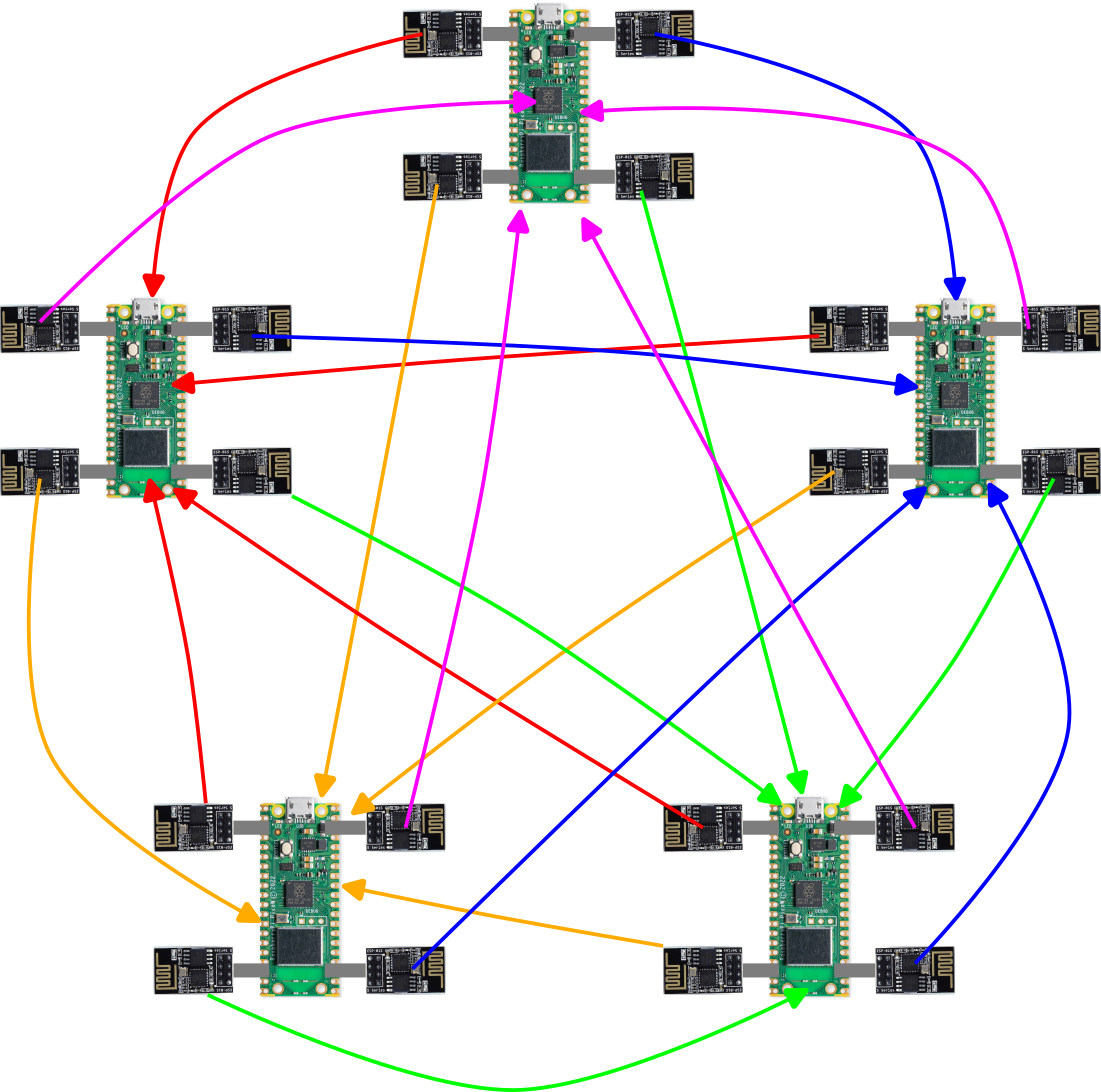
\includegraphics[width=0.8\linewidth]{connections}
  \caption{Полносвязная mesh-сеть, состоящая из пяти контроллеров Raspberry Pi Pico W, каждый из которых имеет четыре радиомодуля ESP-01 (плюс свой собственный). Каждая стрелочка обозначает одно Wi-Fi соединение. Все ESP-01, от которых выходит стрелочка одного цвета, подключены к точке доступа, которая создается контроллером, на который указывает стрелочка. Информация двигается по направлению стрелочки.}
  \label{fig:connections}
\end{figure}


\subsection{Геометрия симулятора}

Наш симулятор сделан в контексте задачи мультиагентного планирования,
и для упрощения логики планнера,
обычно такие задачи имеют дело с дискретным миром.
Кроме того, при переносе этой реализации на физических роботов,
они должны понимать,
в какой точке пространства они находятся.
Из-за этого мы приняли решение,
что роботы двигаются по квадратной сетке,
останавливаясь на пересечениях линий этой сетки.

С точки зрения логики движения, робот может свдинуться вперед или назад на целое количество клеток,
или повернуться влево-вправо на целое количество четвертей.
Это реализуется в физическом роботе посредством датчика линии,
который отслеживает, сколько линий проехал робот вперед
или сколько оборотов он сделал.

Радио-симуляция, напротив, не может работать в дискретных координатах,
потому что распространение радио-сигнала должно быть изотропным,
то есть симметричным относительно вращения~\footnote{Такая модель хорошо описывает антенны общего назначения,
например такие как в Wi-Fi модулях,
но бывают также более направленные антенны.
Наш симулятор может быть использован и с анизотропным профилем уровня сигнала.},
но в дискретных координатах невозможно нарисовать идеальную окружность.
Из-за этого симуляция радио-связи происходит отдельно,
и пока робот двигается от одной клетки к другой,
симулятор постоянно обновляет значение силы сигнала.
Каждый кадр, когда любой робот двигается,
состояние радио-системы будет обновляться.

Из-за этого логика внутри робота разделяется на две части: 
драйвер движения и драйвер радио-коммуникации.
Общение между этими модулями синхронизируется с помощью общей памяти (точнее, примитивов вроде каналов и семафоров, которые основаны на общей памяти),
а большую часть времени они работают независимо.
Это можно обеспечить на многоядерных микроконтроллерах,
таких как Raspberry Pi Pico/RP2040 (наш первый выбор для этого проекта),
или с использованием асинхронных подходов к программированию,
или это тривиально возможно с помощью поддержки множества процессов внутри ядра операционной системы вроде Linux.

\subsection{API для пользовательского кода}

Для разработки симулятора мы решили использовать язык Rust.
Он позволяет нам писать быстрый и безопасный код,
который можно компилировать на многие платформы без изменений~\cite{10.1145/2663171.2663188}.
Благодаря этому симулятор можно запускать как нативное приложение на Linux или Windows,
или как веб-приложение через WebAssembly.

Такое решение также позволяет использовать один и тот же код внутри симулятора
и также на реальном оборудовании --
это потребует лишь написания драйвера для этого оборудования.

Этот драйвер представлен структурой, которая реализует нужный trait (это аналог интерфейса в Rust).
Для поддержки какой-то платформы нужно лишь реализовать соответствующие асинхронные~\footnote{Для embedded-разработки
на Rust используется популярный проект Embassy. С помощью него даже легче писать асинхронные программы
для embedded-платформ, чем синхронные. Это отличается от разработки на Arduino, например,
где ограничения платформы приводят к тому,
что код обычно пишется в синхронном стиле на C++.}
 методы для реализации функционала.

Для управления движением шасси мы можем сами решать, какой интерфейс обозначить,
и в данный момент (как написано раньше)
робот может сдвинуться вперед/назад на несколько клеток или сделать несколько четвертей оборотов
влево-вправо.
У него также есть возможность подождать несколько секунд,
или вывести сообщение для отладки
(оно будет видно только в симуляторе).

Для управления радио-связью мы должны учитывать возможности физического радио-модуля.
В API доступны только те методы,
для которых у ESP-01 есть готовые AT-команды:
например, сканировать соседние Wi-Fi сети,
соединиться с одной из них,
отсоединяться
и измерять уровень сигнала.
Там также есть метод, чтобы отправить сообщение тому роботу,
с которым мы соединены,
в соответствии с моделью радио-связи, описанной выше.
Эти методы описаны в listing \ref{code:traits}.

\begin{listing}[h]
\caption{Описание интерфейса радио-приемника и передатчика.
Драйвер должен реализовать эти два интерфейса,
чтобы быть совместимым с нашим симулятором.}
\label{code:traits}
\begin{minted}[fontsize=\footnotesize]{rust}
/// Интерфейс приемника сообщений (Wi-Fi AP).
pub trait ReceiverNic<PeerId, MessageType> {
    type Error: core::fmt::Debug;
    /// Получить одно сообщение, которое было отправлено на этот приемник.
    /// У драйвера ограниченный буфер для сообщений, поэтому
    /// если это вызывается редко,
    /// то некоторые сообщения могут быть потеряны.
    ///
    /// Асинхронно блокирует, пока сообщение не получено.
    async fn get(&mut self) -> Result<(PeerId, MessageType), Self::Error>;

    /// Получает ID (например, MAC-адрес) этого приемника.
    /// Отправители будут видеть меня с этим ID.
    async fn get_id(&mut self) -> Result<PeerId, Self::Error>;
}

/// Интерфейс передатчика. Он может отправлять сообщения к одному другому приемнику,
/// но он должен сначала быть соединен с ним.
/// (Wi-Fi STA, подключенный к AP).
pub trait TransmitterNic<PeerId, MessageType> {
    type Error: core::fmt::Debug;

    /// Проверяет, что данный передатчик функционирует.
    async fn ping(&mut self) -> Result<(), Self::Error>;

    /// Получает, к какому приемнику мы подключены.
    async fn get_peer(&mut self) -> Result<Option<PeerId>, Self::Error>;

    /// Получает уровень сигнала текущего подключения.
    /// Уровень сигнала может быть 0, если мы сейчас не в области
    /// доступности приемника.
    async fn get_connection_info(&mut self) -> Result<ConnectionInfo<PeerId>, Self::Error>;

    /// Сканирует доступные приемники. Возвращает количество видимых ID.
    /// Найденные ID записываются в переданный массив.
    /// Если видно приемников меньше, чем в массиве места,
    /// то значение последних элементов не определено.
    async fn scan(&mut self, peers: &mut [PeerId]) -> Result<usize, Self::Error>;

    /// Пытается подключиться к одному приемнику.
    /// Если он в радиусе действия и подключение успешно,
    /// возвращает Ok(()).
    async fn pair(&mut self, peer: PeerId) -> Result<(), Self::Error>;

    /// Пытается отключиться от приемника.
    /// Работает даже если приемник не в радиусе действия.
    /// Если мя не подключены к приемнику, то ничего не делает.
    async fn unpair(&mut self) -> Result<(), Self::Error>;

    /// Отправляет сообщение подключенному приемнику.
    async fn send(&mut self, message: MessageType) -> Result<(), Self::Error>;
}
\end{minted}
\end{listing}

Наконец, две части управления запускаются в отдельных потоках
(с помощью инструментов движка в симуляторе
и через \texttt{\#[embassy::task]} на физической платформе).
Для координации между ними предоставлены методы,
которые позволяют им информировать друг друга о том, что произошло интересное событие
(например, логика движения хочет отправить сообщение другому роботу,
или другой робот успешно доставил сообщение этому).

\begin{figure}
  \centering
  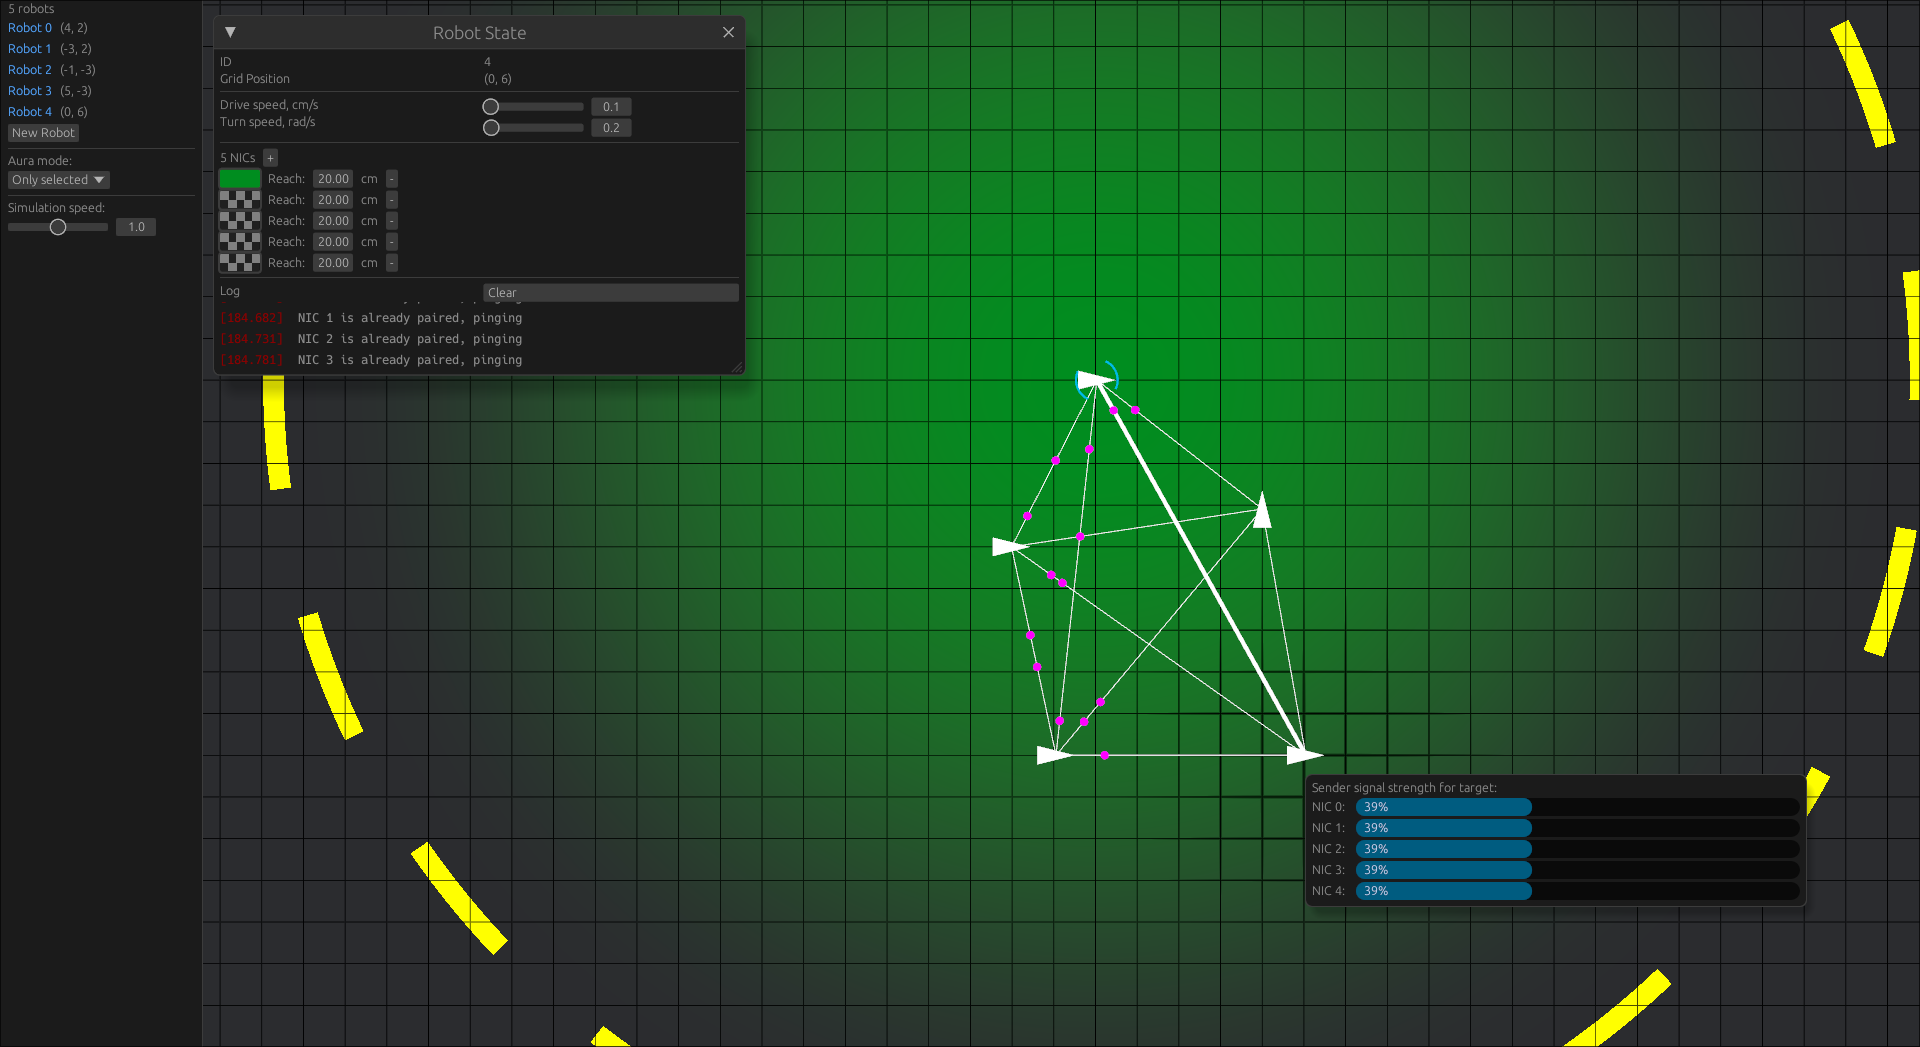
\includegraphics[width=0.8\linewidth]{simulator-connections}
	\caption{Меш-сеть, представленная на рис. \ref{fig:connections}, реализованная внутри симулятора. Каждый робот имеет четыре виртуальных интерфейса, которые позволяют им установить соединение с каждым из соседей. Также на рисунке видна аура и пунктирная окружность вокруг верхнего робота, показывающая радиус действия его радио-интерфейсов; индикатор уровня сигнала, показывающий, что связь между верхним и нижним-правым роботом имеет уровень 39\%. Также видны кружочки на соединениях: это радио-сообщения, летящие между роботами, которые были отправлены, но еще не доставлены.}
  \label{fig:simulator-connections}
\end{figure}


\subsection{Архитектура симулятора}

Поскольку мы выбрали Rust как основной язык разработки,
то мы решили использовать Bevy -- игровой движок на основе модели ECS
(\emph{Entity-Component-System}).
В этой модели существуют сущности (\emph{Entity}),
которые имеют лишь уникальный идентификатор.
К ним привязаны один или несколько компонентов
(\emph{Component}), которые описывают какое-то состояние:
например, в симуляторе используются компоненты,
которые обозначают, что данная сущность является роботом,
который в данный момент двигается от одной клетки к другой.
Наконец, при работе вызываются системы (\emph{System}) --
функции, которые обрабатывают и изменяют данные
в компонентах.

Эта архитектура похожа на ту, которая используется в более популярных
игровых движках вроде Unity~\cite{unity} и Godot;
однако там компоненты и системы
объединяются в одну сущность
(в Unity эта сущность называется \texttt{MonoBehaviour}).
Этот дизайн работает хуже в ситуациях,
когда один код должен действовать над несколькими разными объектами
(например, в симуляциях радио в этом проекте)
и часто требует создания дополнительных виртуальных сущностей
для такой координации.


\section{Заключение}

В данной работе мы разработали симулятор для беспроводных мобильных меш-сетей
и продемонстрировали его API.
На основании этого API можно реализовать алгоритмы, которые будут
работать без изменения кода на виртуальной и аппаратной платформах.
Таким образом мы привносим новизну в область моделирования сетевых архитектур,
в которой раньше большее внимание уделялось задачам моделирования фиксированных сетей.

Из-за гибкости языка Rust,
интерфейс, который мы предоставляем для пользовательского кода,
может быть использован в различных микроконтроллерах.
Благодаря этому мы можем ожидать,
что работа с нашим симулятором станет основой
для будущих меш-архитектурных решений,
поддерживающих разные микроконтроллеры
и физические интерфейсы.

\subsection{Дальнейшая работа}

Наш симулятор предназначен в основном для интерактивного использования,
и он требует графического интерфейса.
Из-за этого он непригоден для ситуаций, когда GUI недоступен,
например на серверах или суперкомпьютерах.
Он также ограничен скоростью симуляции:
многие события требуют, чтобы хотя бы один кадр симуляции прошел
между действием и реакцией
(например: каждая транзакция между кодом радио-модуля
и виртуальным радио-модулем
требует одного кадра,
чтобы быть принятой симулятором.
Из-за этого,
даже если поставить скорость движения сообщений равной бесконечности,
то один робот все равно не сможет передать другому роботу
больше чем 60 сообщений в секунду.)

Эти ограничения связаны с конкретной реализацией симулятора
на основе игрового движка Bevy.
В будущем планируется создать опциональную реализацию,
которая будет работать без графического интерфейса
и обрабатывать события в дискретном времени:
с помощью этой версии можно будет симулировать гораздо более крупные сети.

Для использования в контексте задачи
мультиагентного планирования,
в симулятор будут добавлены
функции для создания дополнительных объектов,
с которыми могут взаимодействовать роботы:
это позволит отслеживать то,
как алгоритм маршрутизации и алгоритм планирования работают вместе.


%Заключение является неотъемлемой частью любой работы. 

%Оно должно содержать краткие выводы по результатам исследования,
%отражающие новизну и практическую значимость работы, предложения по
%использованию ее результатов, оценку её эффективности и качества.

% \section{Ethical disclaimers}

% A disclaimer is a note of disclaimer of responsibility~\cite{kulyabov_2024_editorial_author-ethics_en}.
% For example, authors' statements about conflicts of interest, author contributions, acknowledgements, etc.

% Authors should not prepare these disclaimers as a numbered or unnumbered
% \mintinline{latex}{\section}%
% ; please use the special environments instead.

% \subsection{Author contributions}

% The Committee on Publication Ethics (COPE) draws attention to the problem of authorship \cite{cope_book_authorship_en}.
% The CRediT system (\url{https://credit.niso.org/}) is proposed to formalize author roles.
% The CRediT (Contributor Roles Taxonomy) offers 14 possible author roles \cite{holcombe_2019_contributorship-not-authorship_en}.
% This is not really a taxonomy, but a faceted classification. Author roles are not always independent in themselves.

% The following statements should be used \emph{Conceptualization, X.X. and Y.Y.; methodology, X.X.; software, X.X.; validation, X.X., Y.Y. and Z.Z.; formal analysis, X.X.; investigation, X.X.; resources, X.X.; data curation, X.X.; writing---original draft preparation, X.X.; writing---review and editing, X.X.; visualization, X.X.; supervision, X.X.; project administration, X.X.; funding acquisition, Y.Y.}
% Please add at the end of the statement:
% \emph{All authors have read and agreed to the published version of the manuscript.}

% This section has a special environment:
% \begin{minted}{latex}
% \begin{authorcontributions}
% …
% \end{authorcontributions}
% \end{minted}

% \subsection{Funding}

% Disclaimer \emph{funding} refers primarily to external funding if the research was externally initiated.
% If the research is entirely the initiative of the author's team, it is better to indicate gratitude for partial funding of some of the stages of the research in the \emph{Acknowledgments} section.
% The fact that the author's team has received external funding should be recorded in the disclaimer as a matter of course.
% When mentioning the sponsor, its exact data (name of the organization, grant number, etc.) and the country of its location should be specified (for example \emph{This research was funded by NAME OF FUNDER grant number XXX}).
% If there is any support, it is recommended to clarify in the \emph{Conflicts of interest} section at which stages of the research and how the support was used.
% If there is no external funding, it is written: \emph{This research received no external funding}.
% If it is impossible to obtain information from the authors about the source of funding, then write: \emph{Not specified}.

% This section has a special environment:
% \begin{minted}{latex}
% \begin{funding}
% …
% \end{funding}
% \end{minted}

% \subsection{Data availability statement}

% Data are particularly important in reproducible researches.
% The data availability statement tells the reader where the research data related to the article are located and under what conditions the data can be accessed.
% References to the dataset are also provided.

% If no new data is created or analyzed, please write:
% \emph{No new data were created or analyzed in this study. Data sharing is not applicable.}

% This section has a special environment:
% \begin{minted}{latex}
% \begin{dataavailability}
% …
% \end{dataavailability}
% \end{minted}

% \subsection{Conflicts of interest}

% This disclaimer must be included.

% Conflicts of interest can comment on various aspects, but usually the author's past or current employment is indicated.
% Grants (especially from for-profit companies) received not only by the author but also by the organization for which he or she works are indicated.
% If the author is associated with a sponsor, it is indicated where the research was conducted.

% If there is no conflict of interest, then the corresponding statement should also be included: \emph{The authors declare no conflict of interest}.

% This section has a special environment:
% \begin{minted}{latex}
% \begin{conflictsofinterest}
% …
% \end{conflictsofinterest}
% \end{minted}

% \subsection{Acknowledgments}

% Identification of funding sources and other support, and thanks to individuals and groups that assisted in the research and the preparation of the work should be included in an acknowledgment section, which is placed just before the reference section in your document.

% This section has a special environment:
% \begin{minted}{latex}
% \begin{acknowledgments}
% These are different acknowledgments.
% \end{acknowledgments}
% \end{minted}
% so that the information contained therein can be more easily collected during the article metadata extraction phase, and to ensure consistency in the spelling of the section heading.

% \section{Appendices}

% If your work needs an appendix, add it before the
% \mintinline{latex}{\end{document}}
% command at the conclusion of your source document.

% Start the appendix with the
% \mintinline{latex}{\appendix}
% command:
% \begin{minted}{latex}
% \appendix
% \end{minted}
% and note that in the appendix, sections are lettered, not numbered.

\vspace{\baselineskip}

\begin{authorcontributions}
%  Концептуализация, написание --- рецензирование и редактирование: Анна Владиславовна Королькова; методология, написание --- подготовка первоначального варианта: Дмитрий Сергеевич Кулябов.
Концептуализация, написание --- подготовка первоначального варианта: Генералов Даниил Михайлович;
руководство, написание --- рецензирование и редактирование: Андрей Николаевич Виноградов.
  Все авторы прочитали и согласились с опубликованной версией рукописи.
\end{authorcontributions}

\begin{funding}
  Данное исследование не получало внешнего финансирования.
\end{funding}

\begin{dataavailability}
  В ходе исследования не было создано и проанализировано никаких новых данных. Совместное использование данных неприменимо.
\end{dataavailability}

\begin{conflictsofinterest}
  Авторы заявляют об отсутствии конфликта интересов.
\end{conflictsofinterest}

%\begin{acknowledgments}
%  Мы благодарим организаторов конференции за предоставленную возможность создать этот шаблон.
%\end{acknowledgments}

%%
%% Define the bibliography file to be used
\printbibliography

%%
%% If your work has an appendix, this is the place to put it.
%\appendix

%\section{Онлайн-ресурсы}

%\begin{itemize}
%\item Overleaf: \url{https://www.overleaf.com/read/vjvjpsqrqjhj#86e97e}.
%\item Overleaf (russian): \url{https://www.overleaf.com/read/yjmkpnvgqzdk#bf8ccf}.
%\end{itemize}

\end{document}

%%% Local Variables:
%%% mode: LaTeX
%%% TeX-master: t
%%% End:
